\chapter{Introduction}\label{chap:introduction}

%\section{Motivation}


% Introductory paragraph:
%  Give a general introduction to the topic for broad audience
%  Narrow the focus to your particular topic
%  State your research problem and aims

% hinführung
Tying the shoestrings, running to catch the train, quickly slipping through the closing door and then lifting a heavy suitcase to the luggage rack over the seat\textemdash all actions that are only possible because of the versatility of the musculoskeletal system.
Voluntary contractions of skeletal muscles enable humans to perform a variety of tasks: finely controlled and coordinated actions, endurance tasks, fast and vigorous actions and excercises requiring high forces.

% learn from healthy system and treat diseased system
Moreover, skeletal muscles are able to being trained and adapt to requirements, can self-repair, and usually keep their capabilities for an entire lifetime. Understanding this remarkable system that has evolved over millions of years can advance both engineering and healthcare.

From an engineering view, derived biomimetic systems such as powered exoskeletons or robot arms with muscle-like actuators exhibit promising properties such as being lightweight, inexpensive, resilient, damage tolerant, noiseless, and agile and, thus, are potentially emerging field in robotics and medicine \cite{BarCohen2003,BarCohen2004Electroactivepolymer,Mirvakili2018}.

In the fields of heathcare and medicine, research is interested in obtaining a better understanding of muscular diseases such as muscular dystrophies \cite{Emery2002}. Studies show that disabling inherited neuromuscular diseases are prevalent in 1 out of 3500 of the population \cite{Emery1991}. However, for most of the neuromuscular disorders no cure is known and treatment focusses on reducing symptoms \cite{Emery2002,Heidlauf2015Diss}. Developing treatments to neuromuscular disorders is only possible with an extensive understanding of the neuromuscular system. Similarly, for diagnosing the type of disorder from symptoms and clinically available examination tools such as electromyographic recordings, a comprehensive understanding of muscle physiology is needed.

Surface electromyography (sEMG) measures the temporally changing electric potentials on the skin surface that are induced by activation of the muscles fibers \cite{Merletti2004}. It is one of the few non-invasive diagnostic tools to gain insights into the functioning of the neuromunscular system.
High-density surface EMG (HD-sEMG) involves signal acquisition by an array of electrodes on the skin surface and, thus, enriches the traditional, monopolar EMG by spatial information about the muscular activity. 

Another application where insights into the neuromuscular system advance technology bridges the two fields of engineering and healthcare: Exoskeletons for rehabilitation, e.g., of stroke patients, can be controlled by sEMG or HD-sEMG signals from the patients to accurately support the intended movements (e.g., \cite{Leonardis2015,Mulas2005,Andreasen2005}).

% need for simulation, in-vivo - in-silico
Despite the need to gain comprehensive insights, experimental in-vivo investigations of the neuromuscular system have severe limitations: Boundary conditions, such as contraction velocities often cannot be accurately controlled, studies are not repeatable because of fatigue effects, material parameters of individual subjects are not known and cannot be measured precisely, and the quantities of interest, such as  activation values and active stresses cannot be measured easily. Moreover, experiments are strongly limited to the ethical bounds of natural movements. 

A controlled environment for such investigations can be provided by in-silico experiments, i.e., using computer simulations. The main advantages of using simulations are the unlimited access to all computed quantities, reproducibility, and freedom in the experimental protocol.
With appropriate models, predictions can be made even for pathological conditions.

Employing in-silico experiments demands a careful formulation and composition of mathematical models, using experimentally found evidence about the functioning of various aspects in the muscular system. Once a model is set up, its execution requires suitable numerical methods and an efficient implementation to utilize the available compute hardware in the best way.

%Ich glaube, hier wäre ein Überleitungssatz zum nächsten Absatz gut: Diese Arbeit beschäftigt sich genau mit solchen num. Methoden und deren effizienter Implementierung auf paralleler Hardware. In diesem Kapitel werden Grundlagen eingeführt: .... (Auflistung wie im nächsten Absatz, was in welchem Abschnitt kommt)

This work discusses these numerical methods and their efficient implementation on parallel hardware. The present chapter introduces the fundamentals:
\Cref{sec:anatomy_physiology} presents the basic anatomy and physiology of a skeletal muscle.
\Cref{sec:challenges_in_silico} takes a closer look at the application of the in-silico laboratory and derives requirements on the simulation technology. 
\Cref{sec:intro_related_works} outlines the current state of the art in skeletal muscle simulation. One of the most promising model frameworks that we use is described in more detail in \cref{sec:the_multi_scale_model_of} before contributions of this work are summarized in \cref{sec:intro_contributions}.

\section{Anatomy and Physiology of the Human Skeletal Muscle}\label{sec:anatomy_physiology}

Skeletal muscles have a hierarchical structure as shown in \cref{fig:hierarchical_structure}. On the macroscopic level, fibroelastic tendons connect the muscle to the skeletal system. The muscle is composed of tens of fascicles with the exact number strongly depending on the muscle (numbers according to \cite{MacIntosh2006}). Each fascicle contains between ten and 10.000 muscle fibers, yielding a total of up to one million fibers in a muscle. Each muscle fiber usually runs through the whole length of the muscle. A muscle fiber consists of numerous parallel myofibrils which each consist of series of sarcomeres, the smallest contractile unit of a muscle. A muscle fiber contains approximately 50.000 sarcomeres and, thus, there are from millions up to billions of sarcomeres in a whole muscle.

\begin{figure}
  \centering%
  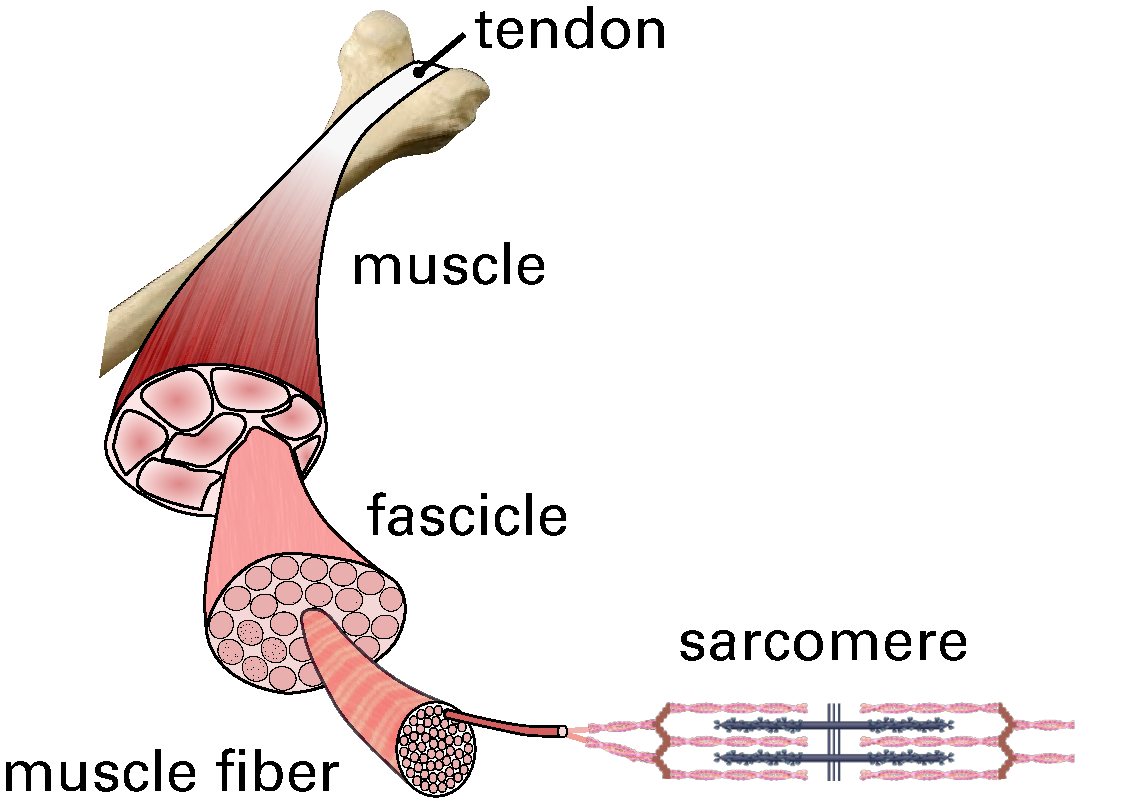
\includegraphics[width=0.5\textwidth]{images/introduction/hierarchical_structure.pdf}%
  \caption{Hierarchical structure of a skeletal muscle consisting of fascicles, muscle fibers and sarcomeres.}%
  \label{fig:hierarchical_structure}%
\end{figure}%

Contraction of the muscle is controlled by motor neurons in the spinal cord. The axons of each alpha motor neuron innervate multiple fibers in the muscle. In consequence, all connected fibers are always activated simultaneously. The set of fibers together with their motor neuron form a motor unit (MU).

The neuromuscular junctions where the axons innervate the muscle fibers are mostly located in a band within the midbelly of the muscle \cite{Childers2004}. Upon activation of a muscle fiber, an electric stimulus, the action potential, travels from the neuromuscular junction towards both ends of the muscle. The action potential triggers subcellular processes and leads to force generation in the sarcomeres. The fibers are electrically isolated to each other but mechanically coupled through the fascicles and the extracellular matrix.

The propagation of action potentials is governed by ionic currents through ion channels in the fiber membranes and is driven by ion pumps and the activation and deactivation of the ion channels. \Cref{fig:action_potentials} shows the shapes of two subsequent action potentials over time at a fixed point on a muscle fiber. The transmembrane potential $V_m$ initially equals its resting state of $\SI{-75}{\milli\volt}$. After stimulation occurs, the potential rapidly depolarizes to a maximum value of approximately $\SI{30}{\milli\volt}$, followed by the repolarization and a small overshoot, before returning to the resting potential. After approximately $\SI{30}{\milli\second}$, the system is again in equilibrium and the action potential induced by the next stimulus has the exact same shape.
 
% action potential over time
\begin{figure}
  \centering%
  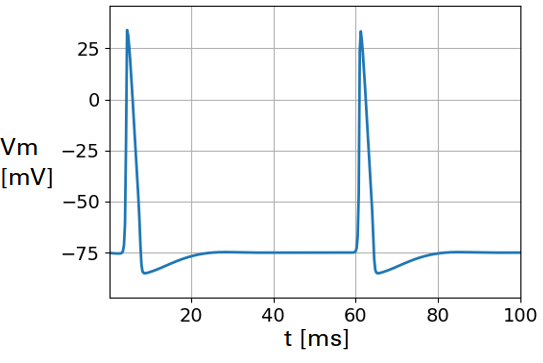
\includegraphics[width=0.6\textwidth]{images/introduction/action_potentials.png}%
  \caption{Action potentials over time at a fixed point on a muscle fiber, calculated by the monodomain equation with a subcellular model of Hodgkin and Huxley using the software OpenDiHu (More details are given in later sections.).}%
  \label{fig:action_potentials}%
\end{figure}%

%The muscle cells that form a skeletal muscle are the muscle fibres. They are bundled to fascicles whereas the whole muscle
%consists of multiple fascicles, as depicted in \cref{fig:muscle}. Tendons connect the ends of a muscle to the bones.
%Inside each muscle fibre multiple long myofibrils are responsible for the force generation.
%They consist of chains of sarcomeres which are the contractile elements of the cell.
%Multiple layers of parallel sarcomere chains areare arranged side by side, triangular in radial direction.

%The sarcomeres consist of thin filaments of the molecule actin and interleaved thick filaments out of myosin, as depicted in \cref{fig:sarcomere}.
%The thick filament contains myosin heads that can bind to the thin filament.
%In a multistep process called \say{crossbridge cycling} this binding occurs, subsequently the angle in which the head is attached changes and leads to a relative motion of the thin and thick filaments after which the head detaches again.
%Involved are, among others, calcium ions and adenosine triphosphate (ATP) which supplies the needed chemical energy.

The MUs are activated according to the size principle starting with the smallest ones that connect to the least fibers and successively adding larger MUs \cite{Milner-Brown1973b}. The amount of muscle activation is controlled by the number of MUs and the rate-encoded stimulation signals for every MU. This finely controlled level is further modulated by the feedback loops of the neuromuscular system. Sensory organs located within the muscle sense stretch, contraction velocity and forces and influence the motor neuron pool.
A more elaborate description of the anatomy and physiology of the neuromuscular system can be found in the book of MacIntosh et al. \cite{macintosh2006skeletal}.

Considering the origin of EMG signals, all action potentials on the muscle fibers contribute to the electric potential in the muscle volume. While electric conduction is directed inside the muscle fibers, anisotropic conduction occurs in the volume of extracellular space. In addition, electric conduction in adipose tissue above the muscle belly influences the electric potential on the skin surface, which can be measured by EMG.

\section{ Use-Cases and Requirements for Simulations Used in in-Silico Experiments}\label{sec:challenges_in_silico}

With a basic understanding of the physiology of the neuromuscular system, we can now define use-cases for in-silico experiments and derive the requirements for models and simulation software.

A simulation should be able to accurately predict the response of the neuromuscular system to different recruitment strategies of the MUs. 
Also, different organizations of muscle fibers in MUs could be investigated. Similarly, the sensory feedback loop within a single muscle is by far not yet fully understood. Various assumptions could be tested in simulations and the resulting force and EMG outputs could be compared to experiments. By  complementing in-vivo and in-silico experiments, more comprehensive insights can be generated.

A second use case for simulations of the neuromuscular system lies in the decomposition of EMG recordings. Traditionally, signal processing techniques are used to draw conclusions from EMG data \cite{Merletti2004,Farina2010}. Decomposition algorithms exist that identify discharge patterns of individual motor units in HD-sEMG and additively decompose the recording \cite{DeLuca2006,Nawab2010,holobar2007gradient}. 
Novel, data-based techniques exist that employ deep learning methods \cite{Clarke2021}.

However, these techniques have limitations. The recorded signals are typically weak and noisy because of the layer of body fat between the muscle and the EMG electrodes. Cross-talk from adjacent muscles and destructive interference between signals of spatially close muscle fibers make the decomposition more difficult. Often, only isometric contractions can be considered in experiments since large movements of the muscles with respect to the electrodes would add additional uncertainties to the recorded signal.

Simulations can provide a controlled testing environment for such EMG decomposition algorithms. For data-based methods, simulations are unavoidable to generate training and validation data.

The listed use-cases for in-silico experiments demand for detailed, biophysically informed models. Phenomenological descriptions cannot predict unseen scenarios or pathological conditions. The hypotheses to test related to MU organizations, recruitment or sensory feedback have to reflect in the choice of the model description.
A suitable model usually needs to take into account the multi-scale nature of the neuromuscular system. The geometric structure of muscle fibers embedded in the muscle belly and the layer of adipose tissue  have to be part of accurate models.

Multi-scale multi-physics simulations with high resolutions involve high computational loads. The simulated processes on a molecular scale, e.g., in the sarcomere require small timestep widths in the range of microseconds. At the same time, macroscopic quantities such as EMG signals and muscle contraction should be computed, leading to desired overall simulation time spans in the range of seconds.
Fine three-dimensional (3D) meshes are needed to achieve high spatial resolutions. To resolve individual muscle fibers, additional one-dimensional (1D) fiber meshes are considered.

To account for fine resolutions and a high number of timesteps in an acceptable runtime, the potential of todays and tomorrows computer hardware has to be fully exploited. This requires task-level and instruction-level parallelism. For example, the latest processor of the Intel Core X series (the Intel Core i9-10980XE Extreme Edition Processor), which is listed at a customer price below \SI{1000}[\$]{} contains 18 hardware cores, allowing to run 16 tasks in parallel. It supports Intel AVX-512, a technology with which eight double precision floating point operations can be executed per instruction. 
In a higher price segment it is, e.g., possible to combine two AMD EPYC 7742 server processors into a shared memory compute node with \num{128} cores. Distributed memory clusters allow the combination of almost any number of compute nodes to achieve higher total core counts. The supercomputer Hawk at the High Performance Computing Center Stuttgart combines \num{5632} of the mentioned AMD nodes into an overall cluster of \num{720896} cores.

Thus, a requirement to the simulation software is to be able to run on distributed memory computer systems. This requires efficient data management and a domain decomposition approach where the computational domain is partitioned into one subdomain for each process.
Highly parallel domain decomposition requires appropriately structured meshes and efficient parallel linear solvers. At the same time, muscle geometries obtained from medical imaging should be used to obtain a realistic setting. In a preprocessing step, the required highly resolved meshes have to be generated from imaging datasets.

A highly resolved simulation model can be used to estimate the accuracy of reduced models that do not include all biophysical processes or have reduced spatial resolutions. The advantage of such reduced models is that they can be solved with less resources or in shorter runtimes. To assess the error of the reduced resolution, comparisons with results of the full model can be carried out. In this sense, the full model should be able to be used with a realistic number in the order of several \num{100000} muscle fibers and hundreds of MUs to allow for a comparison with simulations of smaller numbers of fibers.

% numerics
Highly resolved simulations are known to exhibit numerical instabilities, poor conditioning or other causes for divergence in the numerical solvers. Therefore, numerical schemes have to be chosen carefully. At the same time, timestep widths can be increased and runtimes reduced by chosing, e.g., second order timestepping schemes instead of first order schemes.

% flexibility
Another important requirement on the simulation software can be formulated from the user's perspective. 
Configuring a simulation and exchanging material and numerical parameters should be possible in a convenient way. Simulation results should be accessible in various established file formats, to be examined in dedicated visualization software or used in further postprocessing. On the modeling side, comprehensive state-of-the-art models should be implemented while maintaining the possibility to extend given multi-scale models later on as research advances. 
Standards in the biochemical modeling community should be respected and incorporated such as the description language CellML \cite{Cellml2003,Lloyd2004} for subcellular models.
To find the most suited numerical solvers, the software should be flexible enough to, e.g., easily exchange timestepping schemes or employ different linear system solvers.

%  State your research problem and aims
% what we do
Our contribution is to implement and employ software that fulfills all these requirements. We aim at
simulating EMG and muscle contraction with detailed, biophysically informed multi-scale models. The software runs efficiently on the previously described hardware, ranging from workstation computers to supercomputers.

\section{Related Work and Software}\label{sec:intro_related_works}

%Literature review (usually several paragraphs):
%  Summarize the relevant literature on your topic
%  Describe the current state of the art
%  Note any gaps in the literature that your study will address
In the following, we give an overview of existing approaches for modeling the neuromuscular system. The overview involves literature and software frameworks and focuses on the multi-scale model that is the basis for the present work. For a recent, comprehensive review on all aspects of neuromuscular modeling, we refer to \cite{Rohrle2019Review}.

\subsection{Related Work}
The lowest computational effort is required when analytically solvable models are used to simulate skeletal muscle forces. The twitch force of a single motor unit can be described by the impulse response of a critically damped, second-order system, for which an analytical solution exists. For the given superposition of all motor unit action potentials, the transient output force of the muscle is computed  \cite{Cisi2008,Dideriksen2010}.
% muscle control

On the next level of detail, phenomenological Hill-type muscle models, which have to be solved numerically are used to describe muscle forces along a one-dimensional line of action. They are often used for systemic simulations of larger parts of the musculoskeletal system \cite{Zajac1989,OpenSim2007,Hilltype2014,Bayer2017}. We use Hill-type models in our case study on predicting forces of the upper arm. However, this type of model is not suited for simulations of EMG and neglects structural properties of the muscle tissue.

While phenomenological models describe a whole muscle by a small number of parameters, continuum-based models exist that also take into account structural features and spatial heterogeneity \cite{Johansson2000,Blemker2005a,Roehrle2007,Boel2008}.

A commonly used approach to model muscle contraction in continuum-mechanics is to additively compose the stress tensor of a passive and an active stress term \cite{blemker2005three,Johansson2000,Roehrle2008}. The passive muscle behavior can be parametrized using experimentally found relations, though this is challenging in practice \cite{Boel2012,Takaza2013,VanLoocke2008,VanLoocke2006}.

Multi-scale models exist that combine formulations of continuum-mechanics with a description of electrophysiology \cite{Roehrle2008,Roehrle2012,Heidlauf2013,HernandezGascon2013}.
These models couple various physical phenomena that occur on different temporal and spatial scales on cell, tissue and organ levels, such as subcellular ion dynamics in scales of milliseconds and micrometers and mechanical stresses and electric potentials in scales of seconds and multiple centimeters.% on the whole muscle with a length  scale of tens of centimeters.

Model order reduction techniques and surrogate modeling have been applied to these complex, full models to speed up the computations \cite{Mordhorst2017,Valentin2018}.

EMG signals of activated muscles can be computed by volume conductor models \cite{Mesin2013}. Both 
 analytic \cite{Dimitrov1998, Farina2001, Mesin2006} and numerical methods exist \cite{Lowery2002, Mordhorst2015, Mordhorst2017, Klotz2020}.

We combine existing multi-scale models of electrophysiology, muscle contraction and generation of EMG with different subcellular models and electrophysiology formulations as well as motor neuron and afferent feedback models to form a novel, comprehensive multi-scale modeling framework for the neuromuscular system. We solve these models using numerically efficient schemes that are implemented in our unified simulation software environment named OpenDiHu.
 
\subsection{Related Software}\label{sec:intro_related_software}
Few software packages exist in the open source world that can be used for comprehensive multi-scale modeling of the neuromuscular system. In the following, CellML, OpenCMISS, Chaste, FEBio and the generic frameworks OpenFOAM and FEniCS will be briefly evaluated.

A useful and widespread technology for biochemical models is CellML \cite{Cellml2003,Lloyd2004}. The open standard CellML language allows to define differential-algebraic equations with physical units. It can be used to develop mathematical descriptions of biophysical processes such as subcellular or neuron models. The description language has also been used for broader applications, e.g., for constitutive material laws. 

CellML provides an online repository where mathematical models and metadata such as figures and related publications are collected. The models can be downloaded as code in various formats and programming languages. Existing models can be combined into new models in a hierarchical manner. Dedicated modeling environments for CellML models exist. As an example, OpenCOR \cite{OpenCOR2015} can be used to edit, simulate and visualize CellML models. Moreover, application programming interfaces (APIs) exist, which provide low level access to models in CellML format and allow software frameworks to integrate CellML functionality.
Among the software frameworks with CellML support are OpenCMISS and Chaste.

OpenCMISS (Continuum Mechanics, Imaging, Signal processing and System identification) \cite{Bradley2011} provides a set of open source libraries and applications for modeling and visualization of bioengineering problems. The frameworks allows to use CellML models \cite{Nickerson2014}.
OpenCMISS Iron, the computational engine, can solve finite element models, discretized also with higher order elements and using cartesian or curvilinear coordinates. For example, the ventricles of the heart were modelled with a low number of cubic Hermite elements in a prolate spheroidal coordinate frame \cite{smith2004multiscale}.
Various nested timestepping loops and solvers can be configured to create multi-scale models. 

The library is programmed largely in the Fortran-90 standard, wrappers for the Python programming language can be automatically generated. It supports parallel execution on distributed memory systems.

The development of OpenCMISS Iron started in 2005 as a rewrite of the computational modeling tool CMISS, whose history dates back to 1980. It is part of the Physiome Project, an international collaborative open-source effort to provide a public domain framework for computational physiology \cite{Hunter2004}.
OpenCMISS has been used for multi-scale modeling of the lungs and heart \cite{smith2004multiscale}, vascular and thermoregulatory system \cite{ladd2016open,ghadam2020modeling} and skeletal muscle \cite{Heidlauf2013}. 

% Chaste
The "Cancer, Heart, and Soft Tissue Environment`` (Chaste) is an open source C++ library targeted at simulations of physiology and biology in general \cite{Chaste2013}. The code development is driven by cardiac electrophysiology and cancer growth simulations but the framework is also capable of solving  ordinary and partial differential equations from other fields. This involves solvers for CellML models, which have been used to simulate cellular cardiac electrophysiology \cite{ChasteCellML2015}.

Chaste \cite{ChasteCellML2015} also uses the approach of first converting a CellML description into C++ code using the tool \emph{PyCml} \cite{Cooper2006}. Chaste features adaptive timestepping solvers such as the \emph{CVODE} solver from the \emph{SUNDIALS} package \cite{cohen1996cvode} and infers analytic Jacobians from the model equations. The CellML support of Chaste targets \say{automated use} by automatically infering standard variable names, e.g., for membrane voltage and stimulation current.

While cardiac and skeletal muscle tissue are similar with respect to their multi-scale structure, significant differences exist regarding electrophysiology and recruitment of MUs. On cardiac tissue, propagation of action potentials occurs uniformly on a three-dimensional domain whereas in the skeletal muscle a multitude of electrically isolated one-dimensional muscle fibers are recruited independently.
Thus, significant development efforts are needed to transform a cardiac simulation into a simulation of skeletal muscles.

In contrast to OpenCMISS Iron, Chaste advertises its test-driven development process to ensure code quality, correctness and reusability \cite{Chaste2009}. Similar to Iron, the Chaste code runs in parallel on distributed memory systems and uses external numerics libraries for linear system solvers.
It also implements a solver for 3D incompressible nonlinear elasticity which is needed for simulating muscle contraction. However, this solver is not yet parallelized.

A simulation tool specialized in the field of biomechanics is the FEBio project \cite{Maas2012,maas2017febio}. It provides an advanced finite element solver for continuum mechanics of muscle tissue and implements a well-documented library of material models, from basic to advanced and state-of-the-art models. The most recent version includes graphical pre- and post processing tools. Whereas OpenCMISS Iron and Chaste require some knowledge of programming and command line usage, FEBio can be used right away also by application scientists. 
Unlike OpenCMISS and Chaste, FEBio only runs in parallel on shared memory computers, which makes it unsuited for High Performance Computing. FEBio contains no electrophysiology models. Prescribing different levels of activation at different locations in a muscle currently is only possible by a workaround of defining separate materials for every finite element. However, FEBio is extensible by user-defined plugins and multi-scale models would have to be implemented in this way.

More generic simulation frameworks exist that can also be considered for simulations of the musculoskeletal system.

OpenFOAM \cite{jasak2007openfoam} is a well-known C++ software framework that provides methods for "Field Operation And Manipulation``. It is mainly designed for continuum mechanics problems in the field of computational fluid dynamics and uses the Finite Volume method. This method can also be used to solve nonlinear solid mechanics problems \cite{cardiff2014nonlinear}.

Another established general framework for solving partial differential equations is $\text{FEniCS}$ \cite{alnaes2015fenics}. It provides a high-level Python interface to directly describe the model in variational form using predefined operators. Then, it derives finite element discretizations, which it is also able to solve in parallel.

Advantages of such generic frameworks are their mature and efficient solvers and infrastructure such as output file formats and their comprehensive documentation and support. Disadvantages are the missing domain-specific functionality. For example, no solvers for CellML models exist in OpenFOAM and FEniCS. For FEniCS, all existing parts of the desired multi-scale model would have to be formulated in the unified form language. This task needs a more in-depth understanding of the framework for the special requirements of the complex model, e.g., the dynamic, incompressible, nonlinear solid mechanics muscle contraction model with active stress contribution, for which mixed finite element formulations and possibly special numerical preconditioners and solvers are needed. This relativizes the advantages of the high-level interface.
Furthermore, in generic frameworks, it is more difficult to bring own problem-specific contributions to the core code trunk to make them publicly available and reusable.

Therefore, we select OpenCMISS Iron as starting point for implementing multi-scale models. We use the multi-scale chemo-electro-mechanical model that was introduced in \cite{Roehrle2012} and initially implemented in the software OpenCMISS for the tibialis anterior muscle \cite{Heidlauf2013}. However, this implementation did not fully exploit the parallel capabilities of Iron as it was hardcoded for four processes. We remove this restriction and further improve runtimes of the existing electrophysiology model by implementing second order timestepping schemes.

We evaluate the performance regarding parallel scaling and memory consumption on a supercomputer. While the performance is good for small degrees of parallelism, we see an unavoidable barrier for larger parallelism and High Performance Computing (HPC). This barrier arises due to fundamental design decisions in the memory layout and is difficult to overcome in the existing OpenCMISS Iron code.

Furthermore, some of the functionality we require for our multi-scale framework is not available: Abitrary data mapping between meshes is needed for a 3D muscle domain with embedded 1D fibers. Output files use a text-based format that is not suited for HPC, established parallel file formats such as defined by VTK or ADIOS are not available. The nonlinear mechanics solver can only solve static problems. At the same time, the implementation assumes generic coordinate frames and element shapes, which are not necessarily needed in our models. Due to the lack of modern programming language features such as object-orientation and polymorphism, it is very difficult to extend the solid mechanics solver to a fully dynamic formulation.

Therefore, we move the existing models to the new code base "OpenDiHu`` and expand the multi-scale framework by new model components. This gives us the flexibility to implement all requirements listed in \cref{sec:challenges_in_silico} and target towards HPC from the beginning. For compatibility, OpenDiHu can write the same output file format as OpenCMISS. Furthermore, an adapter in OpenDiHu allows to integrate the FEBio mechanics solver with the electrophysiology solver of OpenDiHu.

% our multi-scale approach:
\section{The Multi-scale Model of the Neuromuscular System}\label{sec:the_multi_scale_model_of}

Next, we briefly describe the existing multi-scale model framework that we base our work on.
The chemo-electro-mechanical model was introduced by \cite{Roehrle2012} and described in more detail in \cite{Heidlauf2013} and \cite{Heidlauf2015Diss}. It has been used to investigate different muscle fibers lengths \cite{Heidlauf2014} and later was enhanced by also modeling actin-titin interactions \cite{Heidlauf2016}. The work of \cite{Mordhorst2015} extended the framework by a description of EMG signals.

This model reflects the structural and functional aspects of skeletal muscle tissue and describes its mechanical and electrophysiological properties. Different biophysical processes are realized by sub-models that are linked together to form the overall multi-scale and multi-physics model.

\begin{figure}
  \centering%
  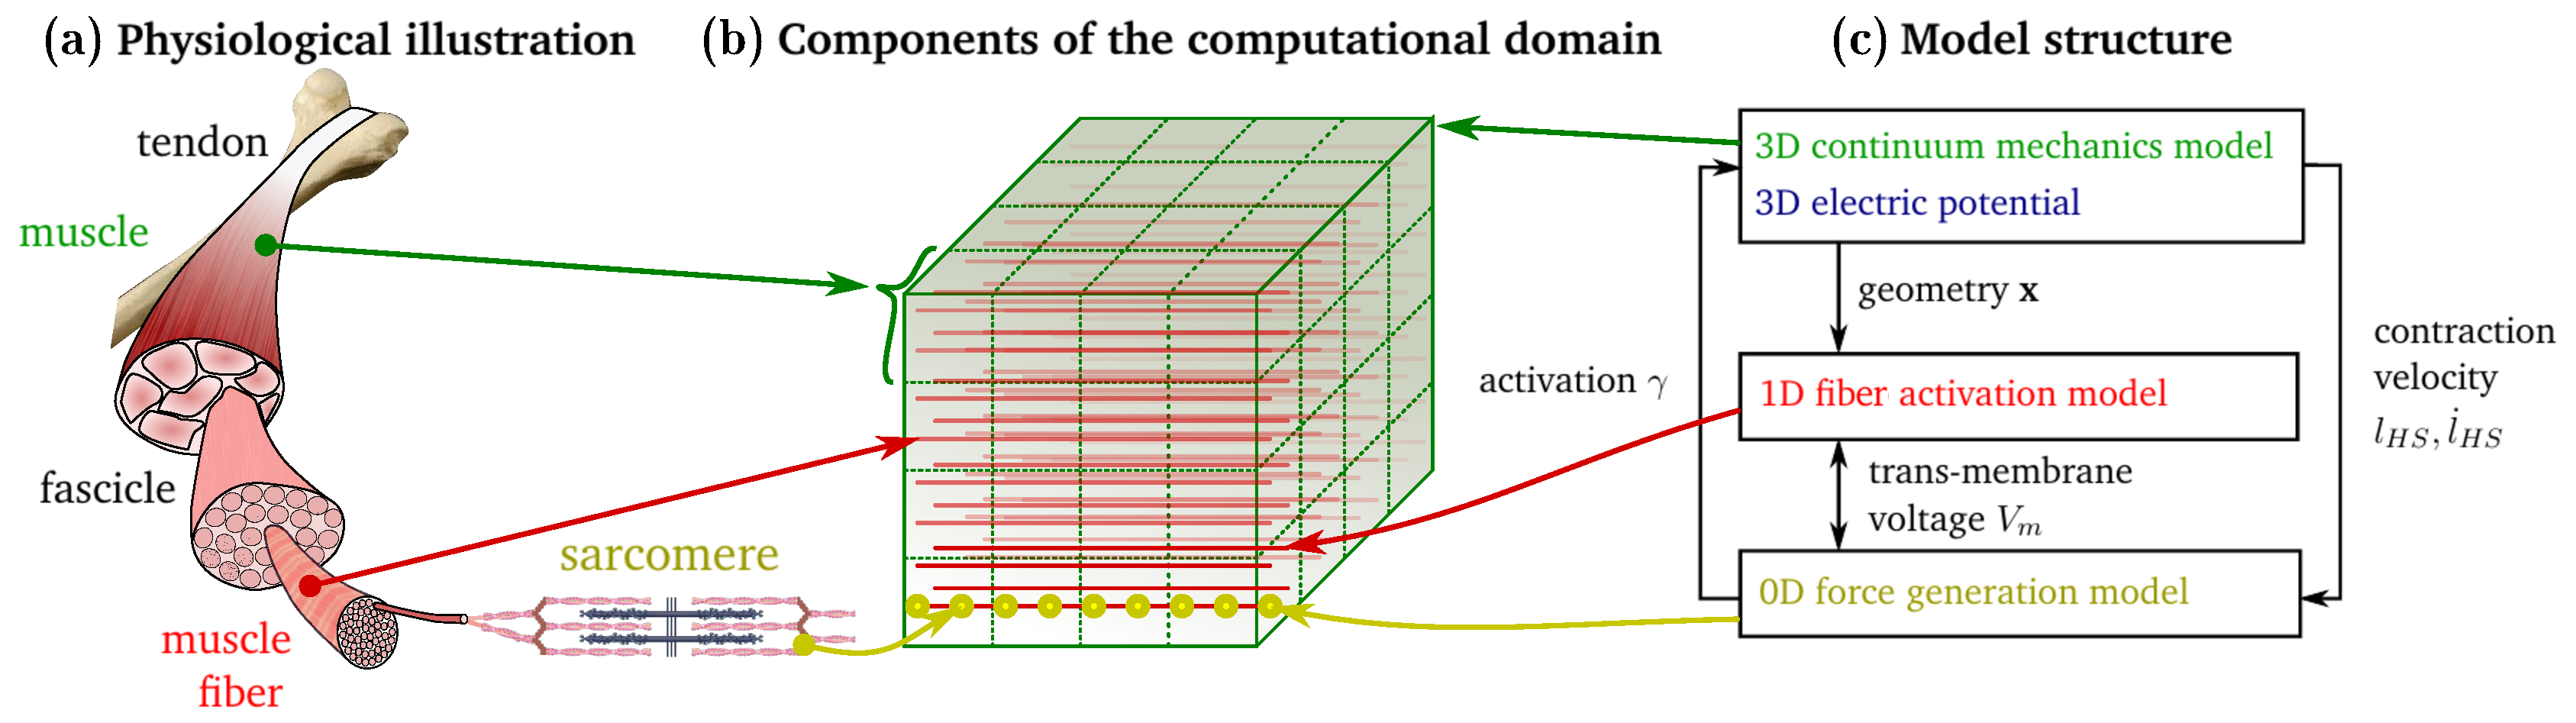
\includegraphics[width=\textwidth]{images/introduction/model_scheme_overview.pdf}%
  \caption{Modeling skeletal muscle physiology: From the anatomy (a) over a multi-scale discretization (b) to the multi-physics model (c) of \cite{Roehrle2012}.}%
  \label{fig:model_scheme_overview_full}%
\end{figure}%

\Cref{fig:model_scheme_overview_full} visualizes the model structure. \Cref{fig:model_scheme_overview_full} (a) depicts the hierarchical skeletal muscle anatomy consisting of muscle, muscle fibers and sarcomeres. \Cref{fig:model_scheme_overview_full} (b) shows the finite element discretization of these three scales. The muscle is represented by a 3D mesh of hexahedral elements (green). Muscle fibers are modeled as 1D fiber meshes (red) that are embedded in the muscle domain. The nodes of the fiber meshes are locations of 0D sarcomere models (yellow). \Cref{fig:model_scheme_overview_full} (b) depicts them only for one fiber, however, the nodes of all fibers feature instances of this model. The cube-shaped 3D domain was chosen for the sake of a clear visualization, our simulations use real muscle geometries instead.

\Cref{fig:model_scheme_overview_full} (c) shows details of the model parts and their exchanged physical quantities. In summary, the model consists of 3D, 1D and 0D components, which are given in different colors.
The green, blue, red and yellow colors are used throughout this work to indicate these sub-models or the three different spatial scales.

The continuum mechanics model describes muscle contraction and is defined on the 3D mesh. The same mesh is also used for computing the 3D electric potential fields within the volume. The deforming 3D muscle domain defines the geometry, i.e., node positions $\bfx$ of the embedded 1D fibers meshes. The 1D fiber activation model computes propagation of action potentials on every fiber. It is strongly coupled via the transmembrane voltage $V_m$ to the 0D force generation model on the sarcomeres which is also called the subcellular model. It depends on the length $l_\text{HS}$ of the half-sarcomere and the contraction velocity $\dot{l}_\text{HS}$. These quantities are computed in the 3D model and mapped to the 0D points. The result of the subcellular model is the activation parameter $\gamma$ that is homogenized and used as input for the active stress term in the 3D continuum mechanics model.

\section{Contributions and Scope of This Work}\label{sec:intro_contributions}

In the following, we give a summarizing preview of the main contributions of this work to the world of existing in-silico models and tools. The contributions include:
\begin{enumerate}[label=(\roman*)]
  \item \textbf{Model extensions.} In addition to the previously existing model components depicted in \cref{fig:model_scheme_overview_full} (c), we add an additional mesh for adipose tissue to simulate EMG signals on the skin surface. The corresponding model was formulated by \cite{Mordhorst2015}, however, it has not been implemented together with the other components in a simulation program prior to our work.

Furthermore, we add the multidomain model \cite{Klotz2020}, an alternative homogenized 3D description of electrophysiology that can replace the 1D fiber activation model and the 3D electric potential in \cref{fig:model_scheme_overview_full} (c). 

Recruitment of the muscle fibers was previously done in a preprocessing step by simulating motor neuron models such as \cite{Cisi2008,Negro2011}. In OpenDiHu, we explicitely couple models of the motor neuron pool as well as models of sensory organs such as muscle spindles and Golgi tendon organs. This allows to close the loop of afferent neural feedback.

Another extension is the consideration of tendons together with the contracting muscle. We add separate models and meshes for the tendons that are mechanically coupled to the muscle belly.

The previous quasi-static mechanics formulation in OpenCMISS Iron is also implemented in OpenDiHu and extended to a fully dynamic formulation. Instead of a numerical approximation of the Jacobian matrix in the nonlinear system in Iron, we automatically derive an analytic description in OpenDiHu. This significantly reduces the runtime and allows to simulate finer meshes than is possible with OpenCMISS.

Current limitations among the implemented models are convergence difficulties for solid mechanics problems with more than approximately 1000 elements. These are not a result of the implementation but a numerical problem and could be addressed by different nonlinear solver schemes in the future.

Whereas the computation using the fiber based description of electrophysiology is close to its optimum performance and scales near-optimally for any degree of parallelism and number of fibres, the corresponding multidomain implementation exhibits high memory consumptions, is less robust with respect to numerical errors and more difficult to parallelize. This restricts its application to approximately 20 motor units, 128 processes and timespans of below a second. If scenarios above these limits are required, the fiber based models should be used.

\item \textbf{Preprocessing Algorithms.} 
A serial and a parallel algorithm are developed to generate the high-quality 1D and 3D meshes that are required for the simulation from imaging data. The algorithms are applied on the biceps and triceps brachii muscles.

Furthermore, a method is derived to assign fibers to motor units according to physiological properties. Both implementations are made publicly available together with the open-source software OpenDiHu.
\item \textbf{Improvements in OpenCMISS Iron.} Improvements include the parallelization to an arbitrary number of cores of the existing implementation of the chemo-electro-mechanical model, an algorithmic improvement from quadratic to linear time complexity in the homogenization functionality of the activation parameter and the introduction of configuration files such that different parametrizations can be simulated without recompiling. Further, numerical experiments concerning employed solvers and timestep widths are conducted. The revised choices, e.g., a conjugate gradient scheme instead of the GMRES solver lead to faster computation times.
\item \textbf{Development of OpenDiHu.} Implementation of an efficient, flexible framework for simulating the full models of surface EMG, muscle contraction as well as subsets of the mathematical multi-scale modeling framework. The software can employ CPUs and GPUs and run on small workstation computers, compute clusters and supercomputers.
As this is the most comprehensive contribution, we refer to the implementation and results chapters, \cref{sec:implementation,sec:results} for details.
Highlights are the simulation of EMG signals with \num{270000} muscle fibers on \num{27000} cores of the supercomputer Hazel Hen and an overall speedup factor of 200 with respect the community standard software OpenCMISS Iron.
\end{enumerate}

\Cref{fig:partitioning_and_full_muscle_emg} shows two snapshots of a simulation that are characteristic for this work: \Cref{fig:partitioning_names} depicts the biceps brachii muscle with a body fat layer. The muscle belly and the fat layer are discretized by nodes and partitioned to multiple processes, indicated by different colors.
\Cref{fig:full_muscle_emg} shows a simulation of EMG signals on the skin surface. Solutions of the  electrophysiology models can be seen on the fibers and on the surface above the muscle.

% Partitioning and Muscle emg
\begin{figure}[H]
  \centering%
  \begin{subfigure}[t]{0.485\textwidth}%
    \centering%
    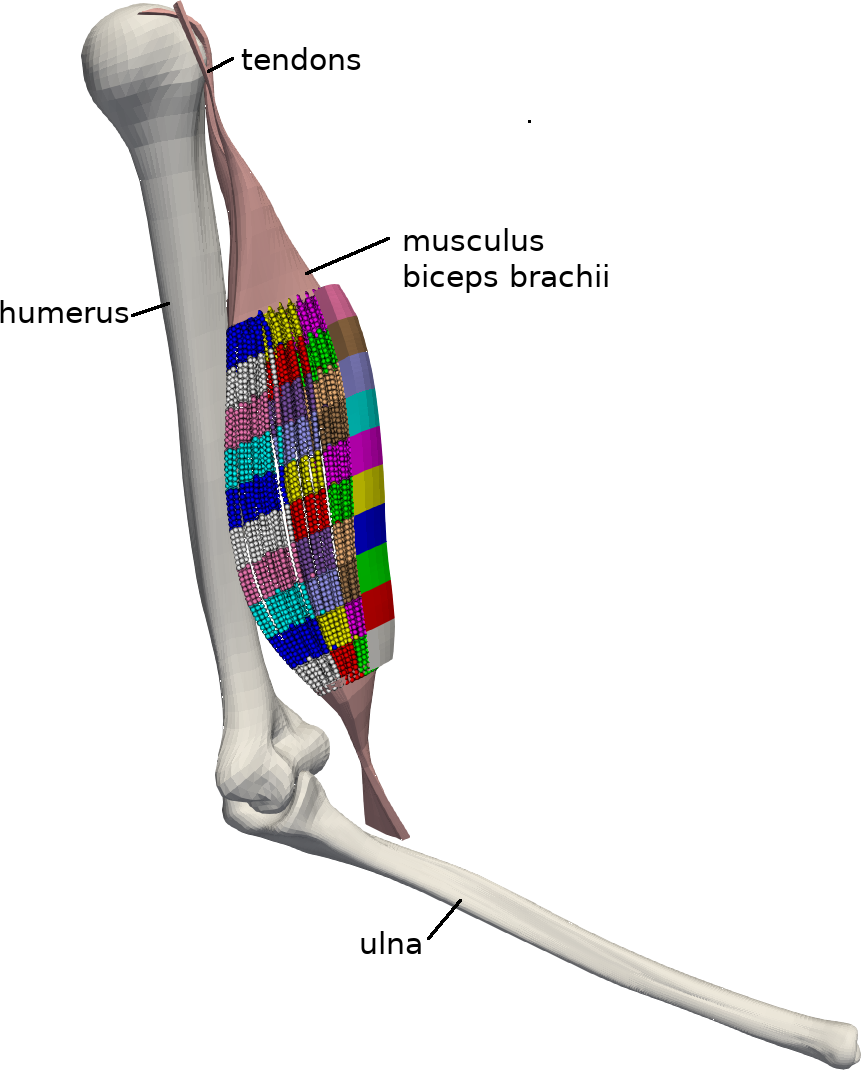
\includegraphics[width=\textwidth]{images/introduction/partitioning_names.png}%
  \caption{The bones of the upper arm with tendons and muscle tissue of the biceps brachii muscle. The colored patches show the domain decomposition of the muscle and of the body fat layer domains.}%
    \label{fig:partitioning_names}%
  \end{subfigure}
  \,
  \begin{subfigure}[t]{0.495\textwidth}%
    \centering%
    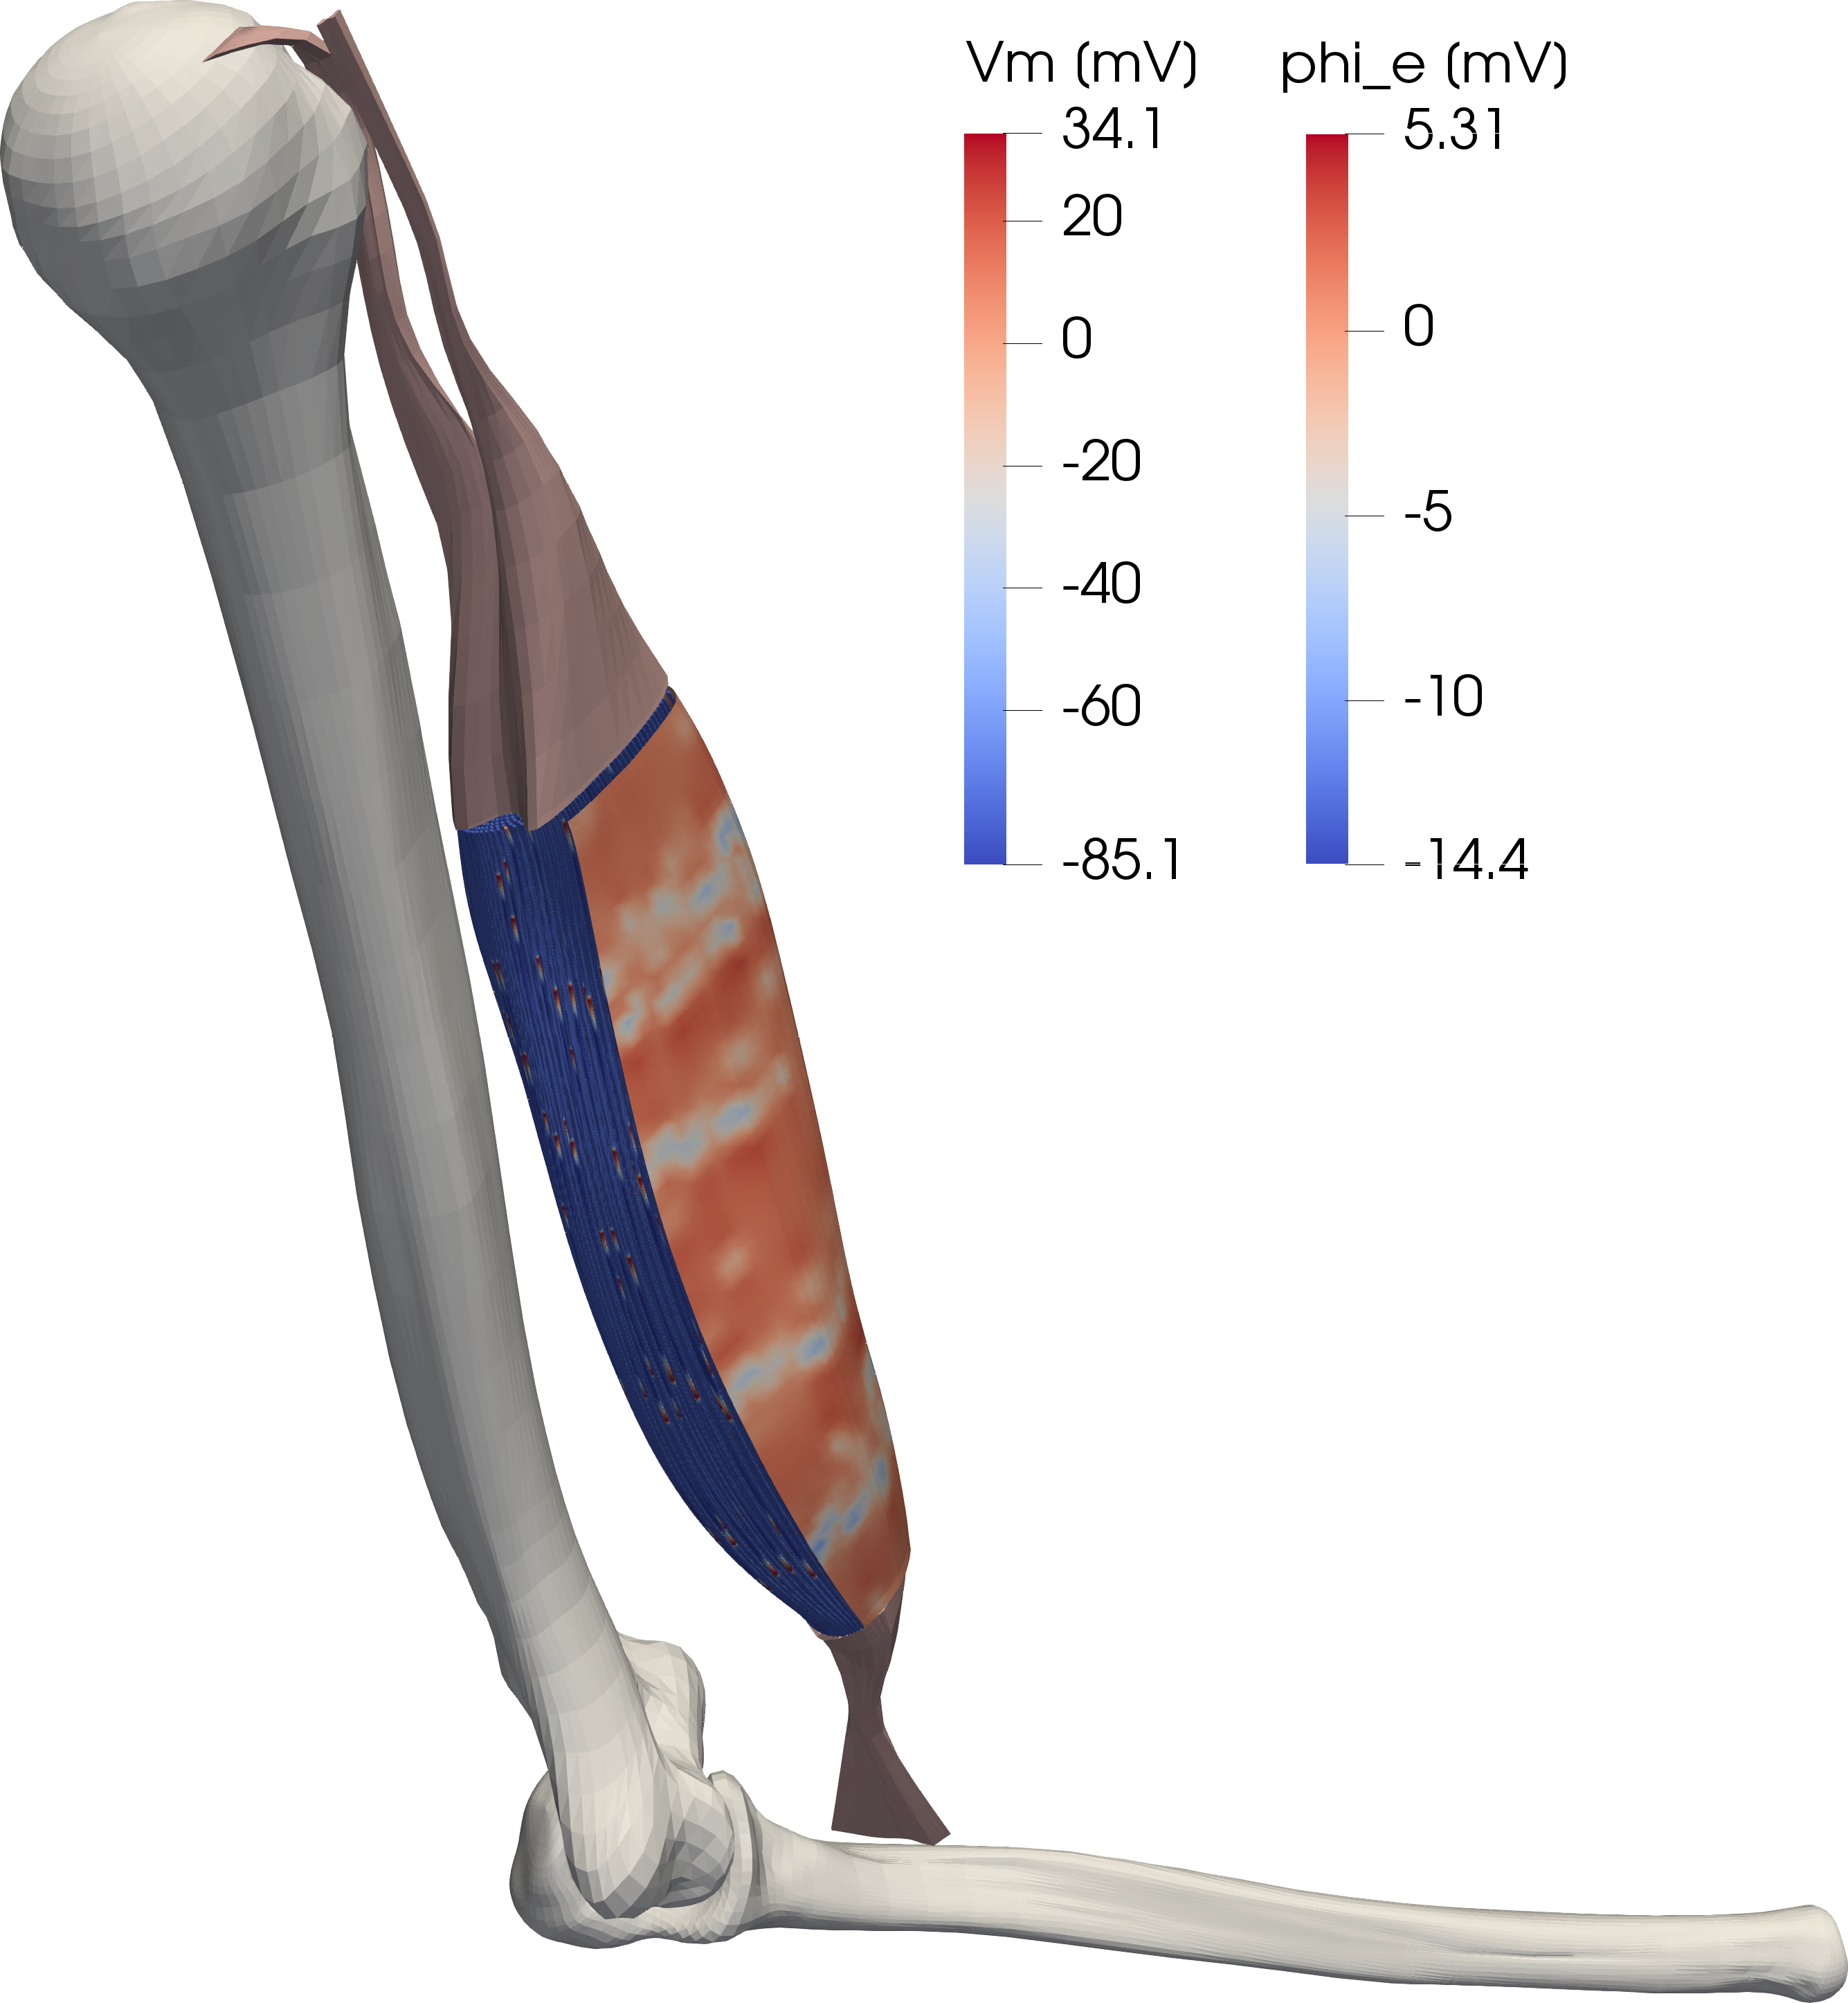
\includegraphics[width=\textwidth]{images/introduction/full_muscle_emg.png}%
  \caption{Simulation of action potential propagation on the muscle fibers (mainly blue, value $V_m$ according to legend) and EMG on the skin surface (value $\phi_e$).}%
    \label{fig:full_muscle_emg}%
  \end{subfigure}   
  \caption{Preview on setting and simulations of a biceps muscle in this work.}%
  \label{fig:partitioning_and_full_muscle_emg}%
\end{figure}%

The scope of this work is to efficiently compute the described models and provide an environment to carry out processing and investigations. The models themselves as well as their parameters are taken from literature. It is known that properties of human organs vary greatly between individuals. For example, the number of muscle fibers in a biceps muscle varies between \num{172000} and \num{419000} \cite{MacDougall1984}.
By parameter fitting, the simulations could be adjusted to represent a particular individual. Within this work, this was done in the initial case study about the upper arm movement for a data-based and a Hill-type based model. However, parameter fitting for the multi-scale model and validation experiments or even pre-clinical studies on patients with musculoskeletal diseases are beyond the scope of this work. Similarly, our software could be used to design studies that foster the understanding of the neuromuscular system. However, such investigations are also beyond the scope of this thesis.

The developed methods in this work were applied to simulations of the biceps brachii muscle, as this muscle allows straightforward EMG recordings and is well-studied in literature. Nevertheless, most of the methods and results are also applicable to other muscles. The anatomical match of the used simulation models could be improved by additionally considering the aponeurosis in the biceps muscle or by differentiating between the two muscle heads during motor unit recruitment. However, these model extensions are also not within the scope of the present work.
Some notes for future work can be found in \cref{sec:future_work}

% explain "we"
The presented findings and conclusions were partly shaped by discussions with various researchers with expertise from different disciplines. Yet, this doctoral thesis lists essentially own contributions, marks collaborative work in the text and indicates others' work by citations.
Using the pronoun \say{we}, the author refers to the group of originator, potentially the supervisors and certainly the interested reader.

% overview of remainder
The remainder of this work contains the following chapters:
\Cref{chap:comparative_study} compares two model approaches to simulate upper arm movement. \Cref{sec:generation_of_meshes_for_multiscale} develops algorithms to generate the meshes that are required in the solution of the multi-scale model. \Cref{sec:muscle_fibers_and_motor_units} addresses the assignment of motor units to muscle fibers. \Cref{chap:models_and_discretization} describes all used model equations and their discretization. \Cref{chap:usage} introduces the software OpenDiHu and describes its usage. \Cref{sec:implementation} gives details on the implementation of OpenDiHu. \Cref{sec:results} presents and discusses numerical results. \Cref{sec:performance_analysis} studies the computational performance of the solvers. \Cref{sec:conclusion_and_future_work} concludes the work and gives an outlook to future work.

%\cref{chap:introduction} % #1 introduction
%\cref{chap:comparative_study} % #2 comparative study
%\cref{sec:generation_of_meshes_for_multiscale} % #3 generation of  meshes
%\cref{sec:muscle_fibers_and_motor_units} % #4 motor units
%\cref{chap:models_and_discretization} % #5 motor units
%\cref{chap:usage} % #6 usage
%\cref{sec:implementation}  % #7 implementation
%\Cref{sec:results} % #8 numerical results and discussion
%\cref{sec:performance_analysis}  % #9 performance analysis
%\cref{sec:conclusion_and_future_work} % #10 conclusion

% ---- end ----



%Research targets (usually one paragraph):
%  State your hypothesis or research question
%  Briefly describe how you will accomplish your aims
%  Give a preview of your main results and state the contribution of the work (optional)

% Contributions
% Limitations (Future Work), Grenzen, Abgrenzung (nicht Gehirn, nicht im Fokus)

%Paper overview (optional; one paragraph):
%  Give a section-by-section overview of the paper's contents
% struktur über weitere Kapitel
% ca. 4-6 Seiten


